\makeatletter
  \graphicspath{ {\import@path} }
\makeatother

\begin{frame}[fragile]{Quark-Gluon Jet Discrimination (1/2)}
  \begin{columns}
    \begin{column}{0.6\textwidth}
      \begin{itemize}
        \item Quark-Gluon Jet Discrimination using Convolutional Neural Network
        \item Jason Sang Hun Lee, Inkyu Park, Ian James Watson, {\bf Seungjin Yang}
        \item \href{https://doi.org/10.3938/jkps.74.219}{J.Korean Phys.Soc. 74 (2019) 3, 219-223}
        \item \href{https://inspirehep.net/literature/1721034}{9 citations}
      \end{itemize}

    \end{column}

    \begin{column}{0.4\textwidth}
      \begin{figure}[htpb]
        \centering
        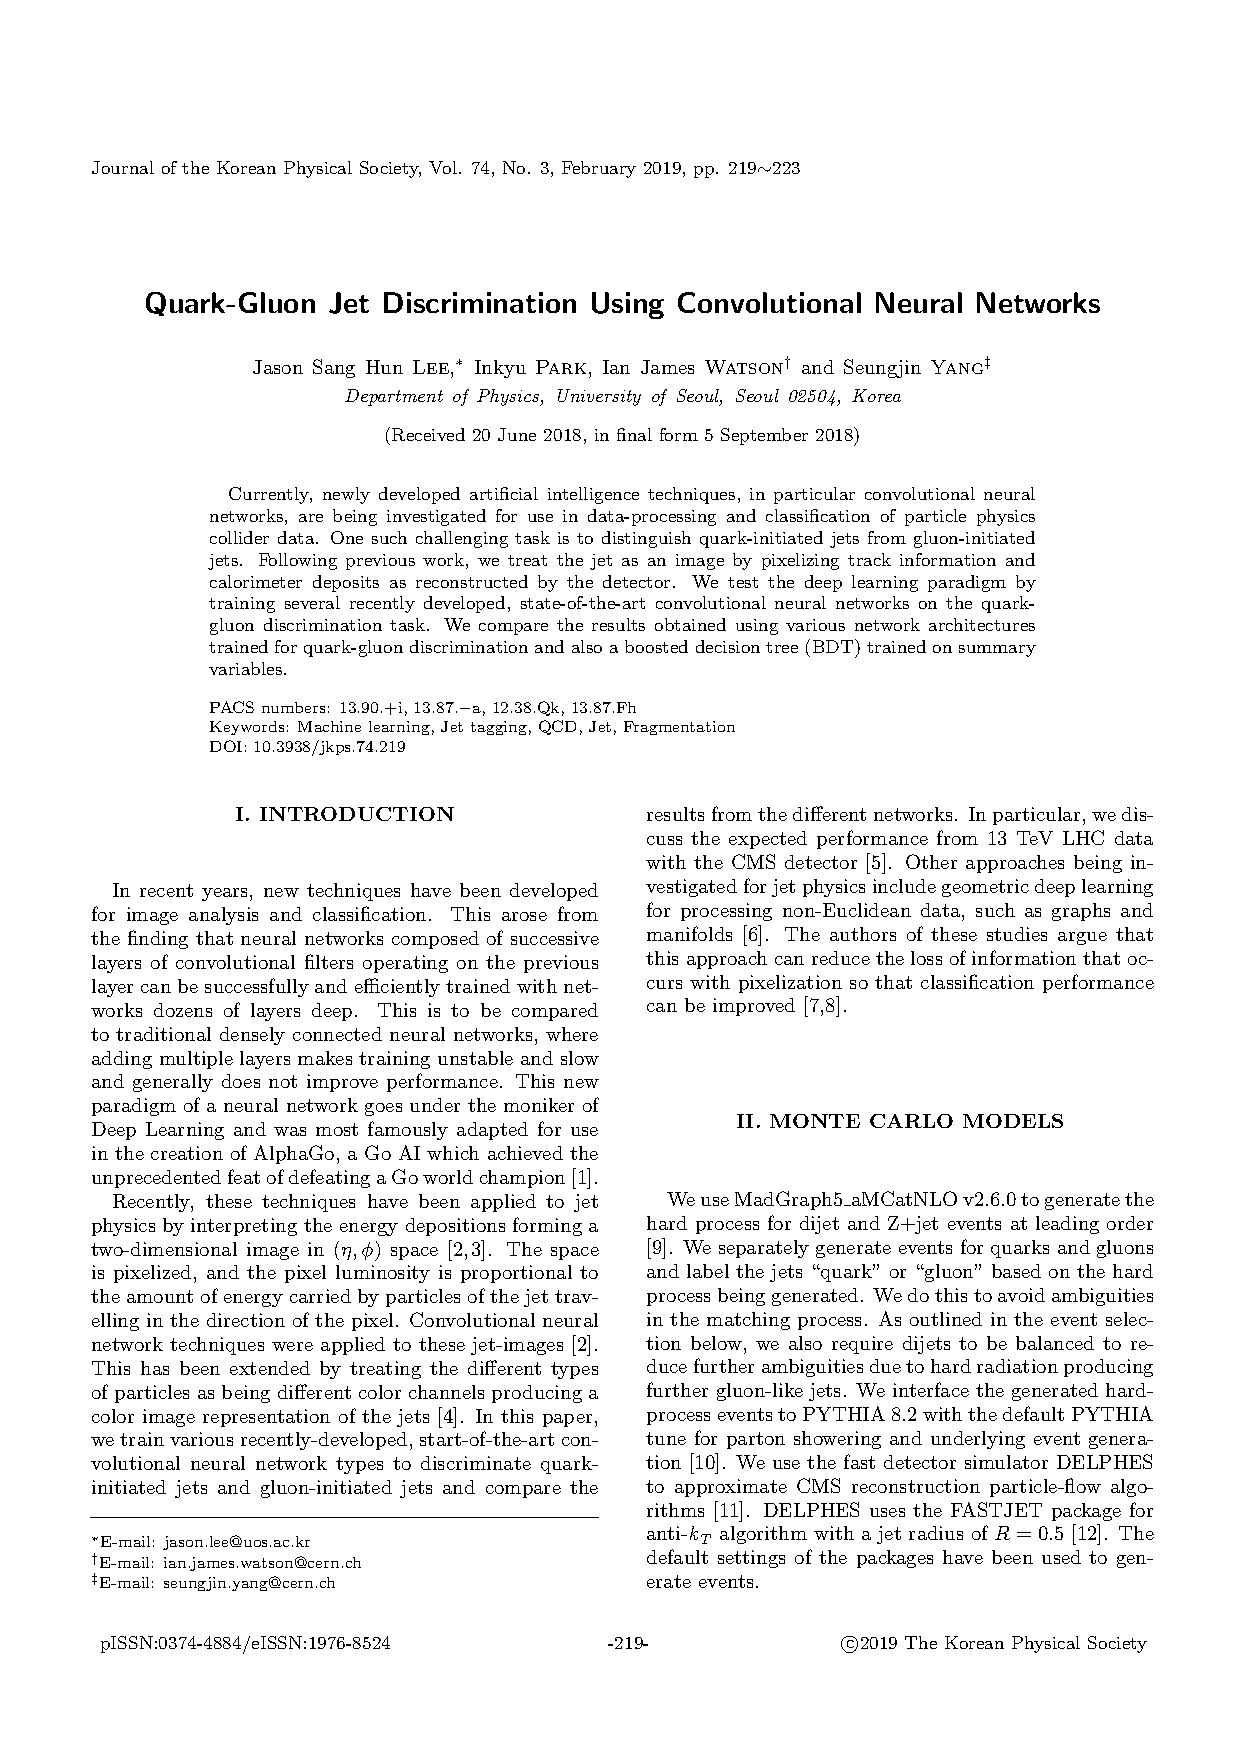
\includegraphics[width=1.0\textwidth]{fig/publication/JP18-0338_F.pdf}
      \end{figure}
    \end{column}
  \end{columns}
\end{frame}


\begin{frame}[fragile]{Quark-Gluon Jet Discrimination (2/2)}
  \begin{columns}
    \begin{column}{0.6\textwidth}
      \begin{itemize}
        \item Quark-Gluon Jet Discrimination using Convolutional Neural Network
        \item Jason Sang Hun Lee, Sang Man Lee, Yunjae Lee, Inkyu Park, Ian James Watson, {\bf Seungjin Yang}
        \item \href{https://doi.org/10.3938/jkps.75.652}{J.Korean Phys.Soc. 74 (2019) 3, 219-223}
        \item \href{https://inspirehep.net/literature/1765363}{7 citations}
      \end{itemize}
    \end{column}

    \begin{column}{0.4\textwidth}
      \begin{figure}[htpb]
        \centering
        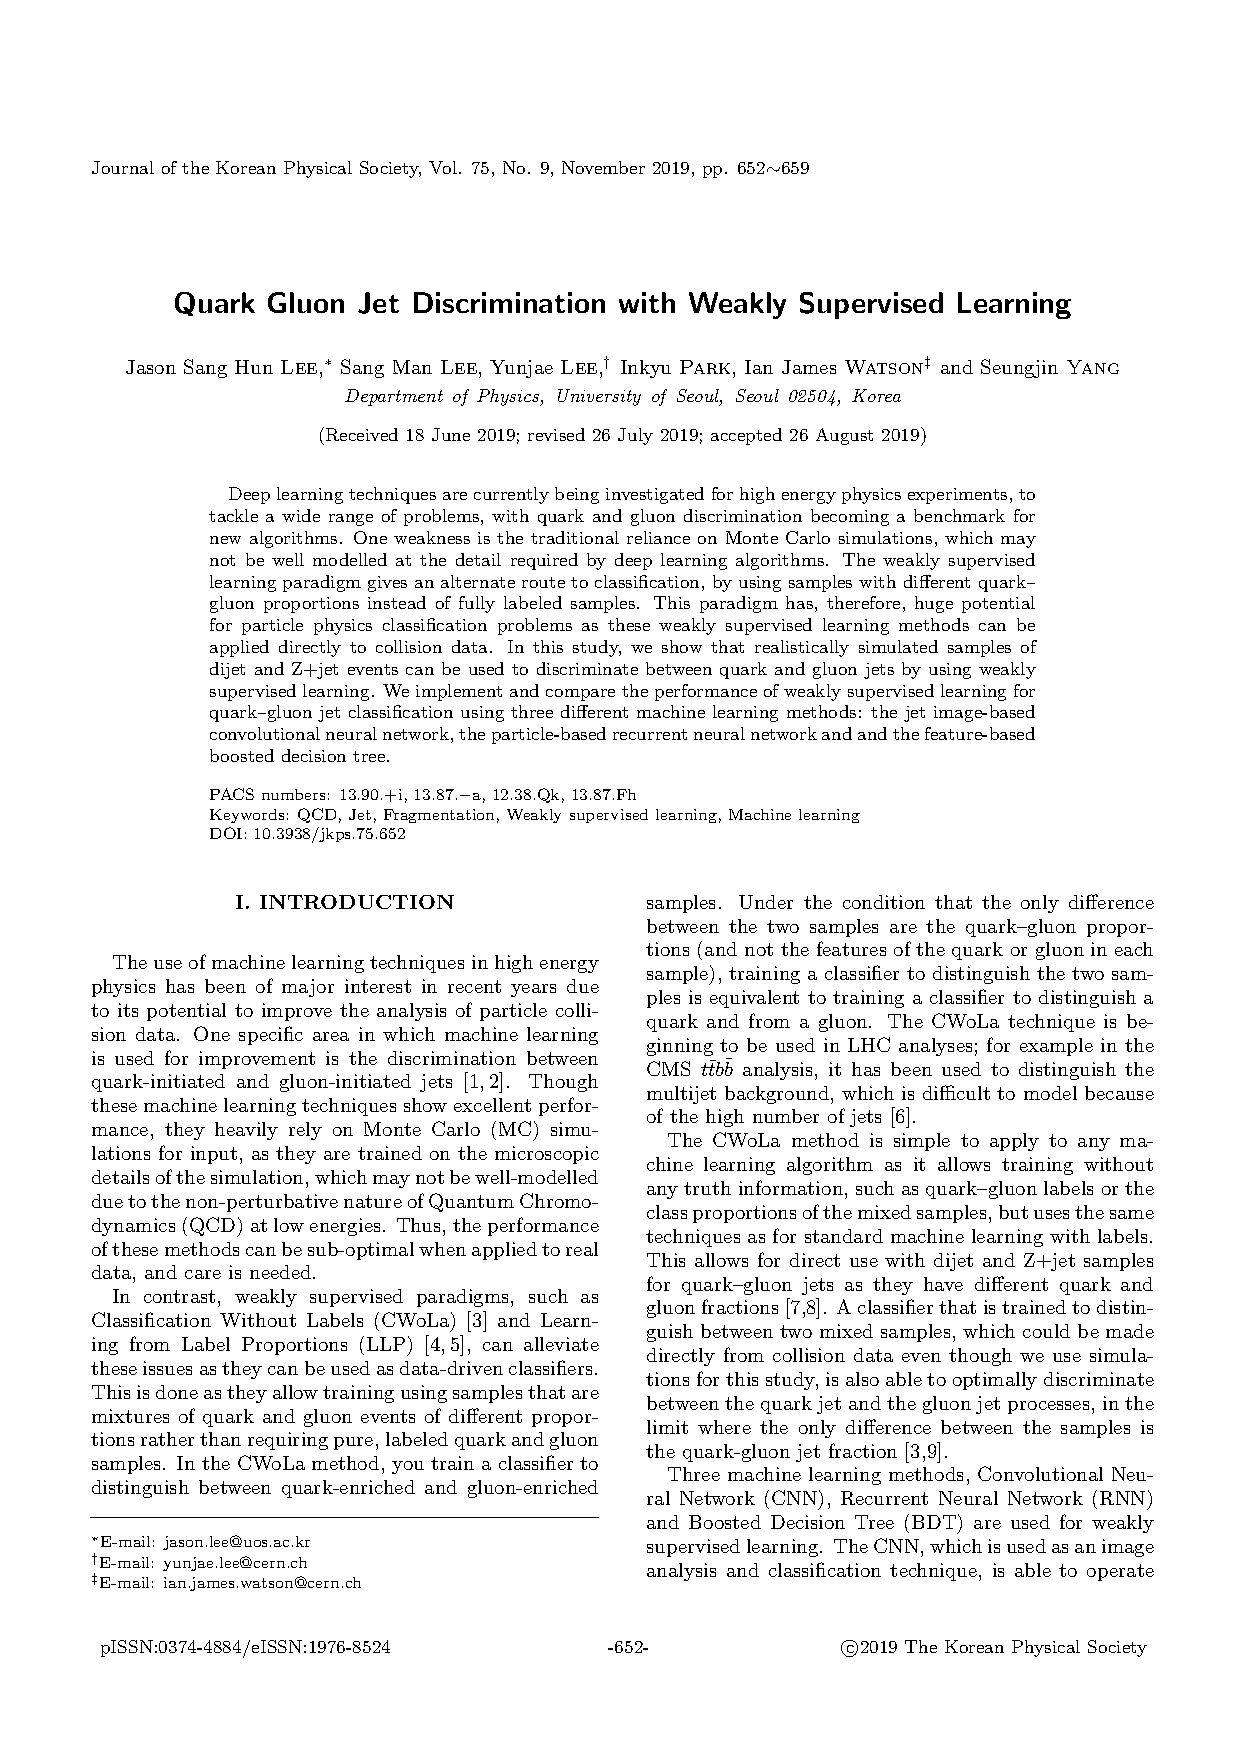
\includegraphics[width=1.0\textwidth]{fig/publication/JP19-0292_F.pdf}
      \end{figure}
    \end{column}
  \end{columns}
\end{frame}
